\documentclass[a4paper]{extarticle}
\usepackage[utf8]{inputenc}
\usepackage[a4paper, margin=1in]{geometry}

\usepackage{amssymb}
\usepackage{amsmath}
\usepackage{enumitem}
\usepackage{tcolorbox}
\usepackage{fancyhdr}
\usepackage{graphicx}
\usepackage{float}

\setlength{\parindent}{0em}
\setlength{\parskip}{0.4em}

\definecolor{theoremblue}{RGB}{1, 73, 124}
\definecolor{corollaryblue}{RGB}{70, 143, 175}
\definecolor{exampleblue}{RGB}{137, 194, 217}

\newtcolorbox{tbox}{colback=theoremblue!20,colframe=theoremblue,
boxrule=0pt,arc=0pt,boxsep=2pt,left=2pt,right=2pt,leftrule=2pt}

\newtcolorbox{cbox}{colback=corollaryblue!20,colframe=corollaryblue,
boxrule=0pt,arc=0pt,boxsep=2pt,left=2pt,right=2pt,leftrule=2pt}

\newtcolorbox{ebox}{colback=exampleblue!20,colframe=exampleblue,
boxrule=0pt,arc=0pt,boxsep=2pt,left=2pt,right=2pt,leftrule=2pt}

\title{IntroML - Lecture Notes Week 2}
\author{Ruben Schenk, ruben.schenk@inf.ethz.ch}
\date{\today}

\pagestyle{fancy}
\fancyhf{}
\rhead{ruben.schenk@inf.ethz.ch}
\rfoot{Page \thepage}
\lhead{IntroML - Lecture Notes Week 2}

\begin{document}

\maketitle
\newpage

\section{Optimization}

\subsection{1D-Case}

The general idea for \textbf{optimization} in 1D is to iteratively try to minimize \(L(w)\):

\begin{cbox}
    \textbf{General iterative algorithm to minimize \(L(w)\)}

    \begin{enumerate}
        \item Start at initial \(w^{start}\)
        \item At each step calculate \(w^{next} = w^{now} + \tilde{\eta} \cdot v\), where \(\tilde{\eta}\) defines how far we move and \(v\) is the update direction depending on \(L\) and \(w^{now}\)
        \item When we can't improve much more, stop
        \item Output \(\hat{w} = w^{final}\)
    \end{enumerate}
\end{cbox}

At each step of the algorithm above, we have to ask ourselves:

\begin{itemize}
    \item Which direction \(v\) should we choose?
    \item How far \(\tilde{\eta}\) to go in that direction?
    \item Can we still improve more?
\end{itemize}

With common sense, if \(L(w)\) decreases as \(w\) increases (i.e. \(L'(w) < 0\)), we should increase \(w\) and vice versa. In other words, we choose the direction \(v = - \text{sign}(L'(w))\).

Choosing \(\tilde{\eta}\) is harder. Generally speaking, we have to decrease \(\tilde{\eta}\) as the slope gets smaller. Even then, \(\eta\) shouldn't be too large because else it can potentially begin to grow again.

Another important question to consider is when do we stop. 

\subsection{Multidimensional Case}

\subsubsection{Visualization of The Loss}

Again, visualization beyond \(d = 2\) is hard, hence our visualizations are for \(w \in \mathbb{R}^2\). Example:

\begin{figure}[H]
    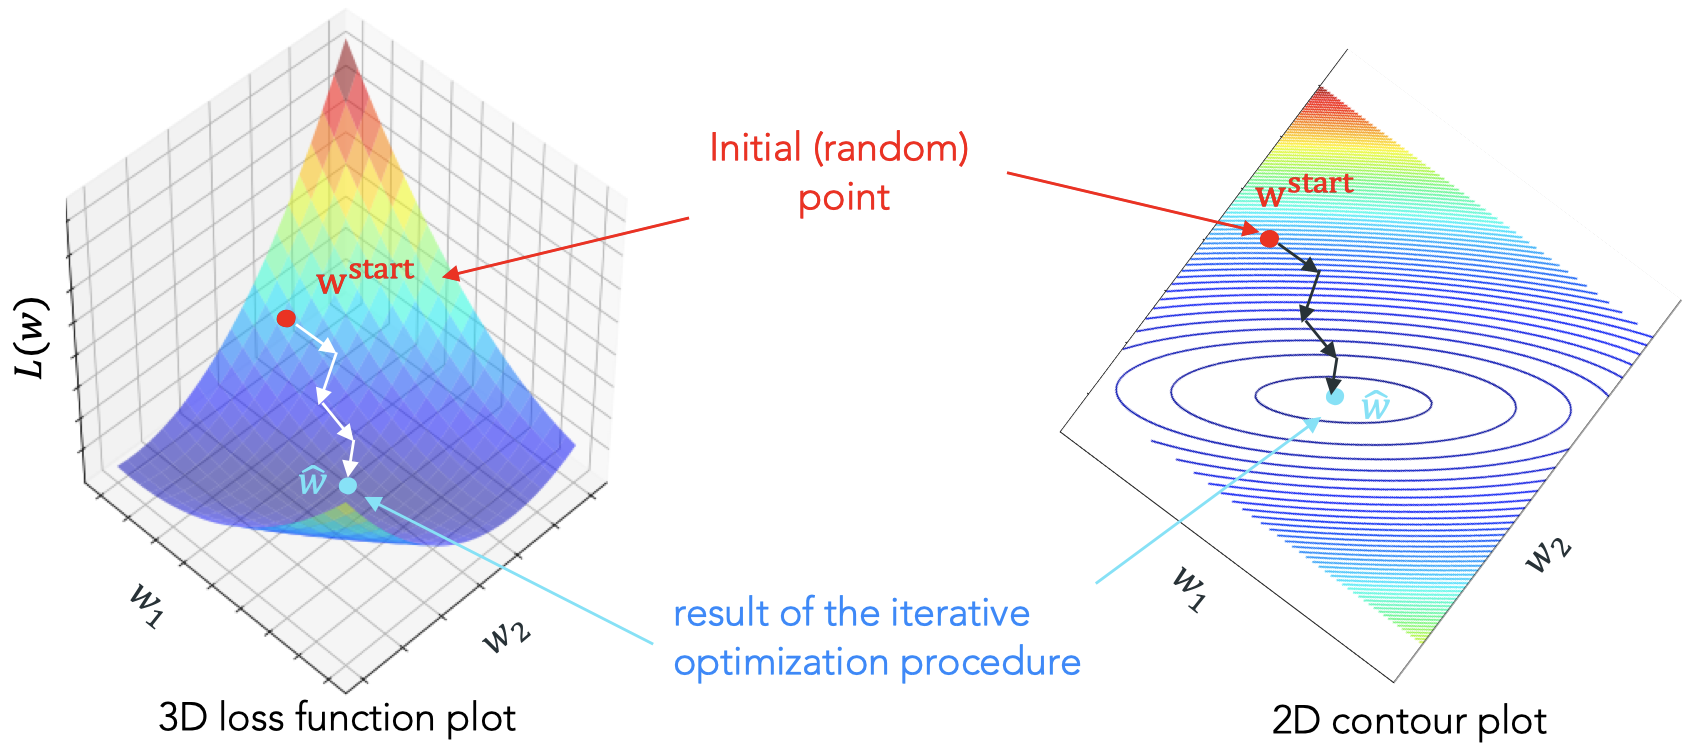
\includegraphics[width=15cm]{../images/IntroML_Fig2-1}
    \centering
\end{figure}

\subsubsection{Steepest Descent}

\begin{figure}[H]
    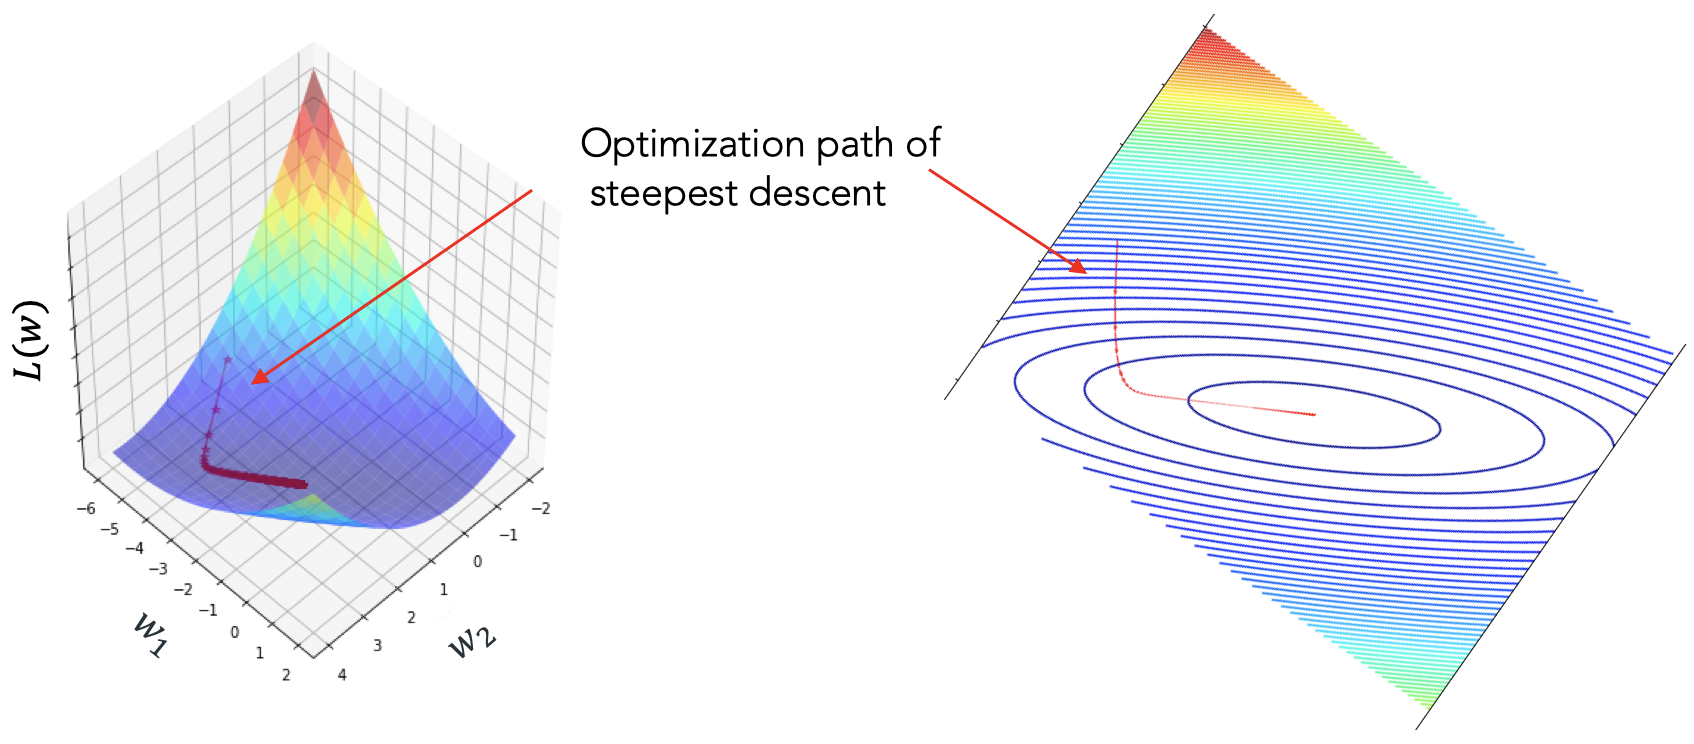
\includegraphics[width=15cm]{../images/IntroML_Fig2-2}
    \centering
\end{figure}

Remember, the general update formula is of the form \(w^{next} = w^{now} + \tilde{\eta}v\) for some unit direction \(||v|| = 1\). What is the \textbf{steepest descent direction} \(v\)?

If we assume that \(L\) is differentiable, then the linear approximation of the loss is given by:

\[
    L(w^{next}) \simeq L(w^{now}) + \tilde{\eta}\langle \nabla_wL(w^{now}), \, v \rangle
\]

The idea is that for small \(\tilde{\eta}\), the steepest direction on the tangent plane is similar to the steepest gradient on the true function. With the derivation of the steepest descent direction on the tangent plane we get \(v = -\frac{\nabla L(w^{now})}{||\nabla L(w^{now}||}\). This leads to the \textbf{gradient descent update:}

\[
    w^{next} = w^{now} - \eta \nabla_w L(w^{now}), \quad \text{with stepsize } \eta = \frac{\tilde{\eta}}{||\nabla L(w)||}
\]

This finally leads to the following algorithm:

\begin{cbox}
    \textbf{Gradient descent algorithm to minimize \(L(w)\)}

    \begin{enumerate}
        \item Start at initial \(w^0\)
        \item Repeat \(w^{t+1} \leftarrow w^t - \eta \nabla_w L(w^t)\)
        \item Stop when \(||w^{t + 1} - w^t|| \propto ||\nabla_w L(w^t)|| \leq 10^{-5} \)
        \item Output \(\hat{w} = w^T\)
    \end{enumerate}
\end{cbox}

The linear approximation for the loss value at step \(t + 1\) is given by:

\[
    L(w^{t+1}) = L(w^t - \eta \nabla_w L(w^t)) \simeq L(w^t) - \eta \langle \nabla_w L(w^t), \, \nabla_w L(w^t) \rangle < L(w^t)
\]

The negative gradient direction is a descent direction (for small enough stepsize \(\eta\))!

\subsubsection{Convergence and Stepsize for Linear Regression}

Remember that for \textit{linear regression} we have \(L(w) = \frac{1}{n} ||y - Xw||^2 = \frac{1}{n}[w^TX^TXw - 2w^TX^Ty + y^Ty]\).

If we use the gradient descent update \(w^{t + 1} = w^t - \eta \nabla L(w^t)\) and if we write \(w_{min} = \text{argmin}_{w \in \mathbb{R}^d} L(w)\). Then indeed, \(w^t \to w_{min}\) and \(||w^t - w_{min}||_2 \leq \rho^t||w^0 - w_{min}||_2\), where \(\rho = ||I - \eta X^TX||_{op}\).

Using the chain rule, the gradient at any \(w\) reads \(\nabla L(w) = -X^T(y - Xw)\), and we obtain \(w^{t+1} = w^t - \eta \nabla L(w^t) = w^t + \nabla X^T (y - Xw^t)\).

If we remember that the global minimum \(w_{min}\) satisfies \(X^TXw_{min} = X^Ty\), then:

\begin{tbox}
    \[
        w^{t+1} - w_{min} = (I - \eta X^TX)(w^t - w_{min})
    \]
\end{tbox}

Furthermore, remember that for any matrix \(A\), \(||A||_{op} = \sup_x \frac{||Ax||_2}{||x||_2} = \max \{|\lambda_{min}(A)|, \, |\lambda_{max}(A)|\}\).

For \(A = X^TX\) this is just the largest eigenvalue. Furthermore, by definition, \(||Ax||_2 \leq ||A||_{op}||x||_2\) and hence:

\begin{tbox}
    \[
        ||w^{t + 1} - w^*||_2 \leq ||I - \eta X^TX||_{op}||w^t - w_{min}||_2 \leq ||I - \eta X^TX||_{op}^{t +1} ||w^0 - w_{min}||_2
    \]
\end{tbox}

If \(\rho < 1 \Leftrightarrow \lambda_{min}(X^TX) > 0\), the error goes to  \(0\) as \(t\) goes to \(\infty\). We say that the \textbf{gradient descent converges linearly / exponentially.}

\subsubsection{Speeding Up Gradient Descent}

To \textit{speed up the gradient descent,} we want large steps in flat areas, and small steps in high curvature ones. This leads to the momentum/accelerated method, where we combine previous direction with the negative gradient direction:

\[
    w^{t+1} - w^t = \alpha (w^t - w^{t-1}) - \eta \nabla_w L(w^t)
\]

\subsubsection{Stochastic Gradient Method (SGD)}

Remember that the training loss definition for parameterized functions is \(L(w) = \frac{1}{n} \sum_{i = 1}^n l(y_i, \, f_w(x_i))\). We have already seen the following algorithm:

\begin{cbox}
    \textbf{Gradient Descent Algorithm}
    \begin{enumerate}
        \item Start at initial \(w^0\)
        \item Until \(w^{t + 1} - w^t\) is sufficiently small, repeat:
        \item \begin{enumerate}
        \item Update \(w^{t + 1} \leftarrow w^t - \eta \nabla_wL(w^t)\)
        \end{enumerate}
        \item Output \(\hat{w} = w^T\)
    \end{enumerate}
\end{cbox}

We see in line 3 of the algorithm above that we need to compute the gradients at all points. This is very costly! The memory required is \(O(nd)\) and the time \(O(n \times \text{cost to compute } \nabla l)\). We propose another algorithm:

\begin{cbox}
    \textbf{Stochastic Gradient Descent (SGD) Algorithm}
    \begin{enumerate}
        \item Start at initial \(w^0\)
        \item Until \(w^{t + 1} - w^t\) is sufficiently small, repeat:
        \item \begin{enumerate}
            \item Update \(w^{t + 1} \leftarrow w^t - \eta \nabla_w L_S(w^t)\)
        \end{enumerate}
        \item Output \(\hat{w} = w^T\)
    \end{enumerate}
\end{cbox}

Here, in line 3, instead of computing the gradient for all points, we only consider a random subset of points \(S \subset [1,..., \, n]\) (so-called \textit{minibatch SGD}). If \(S\) is just one random point, then it's called \textbf{SGD.}

\subsection{Stationary Points and Minima}

Remember that the gradient descent converges to a stationary point, but we want to get to the minimum! For differentiable losses:

\begin{itemize}
    \item \(w\) is local minimum \(\rightarrow w\) is a stationary point
    \item \(w\) is global minimum \(\rightarrow w\) is a local minimum
    \item \(L(w) < L(v) \, \forall v \in \mathbb{R}^d \rightarrow w\) is a global minimum
\end{itemize}

Mathematically, \textbf{convexity} is the function property that guarantees a local minimum to be a global minimum. We have three different conditions:

\begin{itemize}
    \item 0-th order condition (iff.): \(L(\lambda w + (1 - \lambda)v) \leq \lambda L(w) + (1 - \lambda)L(v)\)
    \item 1st order condition (iff.): \(L(v) \geq L(w) + \nabla L(w)^T(v-w)\)
    \item 2nd order condition (iff.): Hessian \(\nabla^2L(w) \geq 0\)
\end{itemize}

Furthermore, we can define a \textbf{strongly convex} functions. We say that \(L(w)\) is strongly convex if \(L(w) - \frac{m}{2}||w||^2\) is convex. We have the following conditions:

\begin{itemize}
    \item 1st order condition (iff. for some \(m > 0\)): \(L(v) \geq L(w) + \nabla L(w)^T(v-w) + \frac{m}{2}||v-w||^2\)
    \item 2nd order condition (iff. for some \(m > 0\)): Hessian \(\nabla^2L(w) \geq mI\)
\end{itemize}

\subsection{Effect of Data on Global Minimum Prediction}

Before we can determine how data affects the model quality, we need to formalize what a good model is:

\begin{itemize}
    \item Goal: Intuition for how the sample size \(n\) can change the prediction performance. What is a good prediction?
    \item Goal standard: Assume the "true" average price is some \textit{ground truth linear function} \(f^*(x) = x^Tw^*\)
    \item Good prediction model \(\hat{f}(x)\): should be close to \(f^*(x)\), i.e. have a low error.
\end{itemize}

When we say that the prediction model should have a \textit{low error,} we mean that:

\[
    l(\hat{f}(x), \, f^*(x)) = (\hat{f}(x) - f^*(x))^2 = ((\hat{w} - w^*)^Tx)^2,
\]

should be low. We often measure:

\begin{itemize}
    \item Average error \(\mathbb{E}(\hat{f}(x) - f^*(x))^2\) over all \(x\), or
    \item for linear functions \(||\hat{w} - w^*||_2\) since \(((\hat{w} - w^*)^Tx)^2 \leq (||\hat{w} - w^*||_2||x||_2)^2\)
\end{itemize}

We often model the observed data as \(y_i = f^*(x_i) + \epsilon_i = \langle w^*, \, x_i \rangle + \epsilon_i\) and call \(\epsilon_i\) \textbf{noise.}

\subsection{Different Dimensionalities}

Let us assume \(n = 2\) points and \(w_0\) to be unknown. There are infinitely many \(w\) that satisfy \(y = \textbf{1}w_0 + Xw\), i.e. that interpolates the training data. If we now assume \(n = 3\) points, for \(d = 2\) there is now only one interpolating solution that satisfies \(y = \textbf{1}w_0 + Xw\).

In general: \textit{the dimensionality of interpolating solutions decreases.}

Again, assuming \(n > d\), we still have infinitely many \(w\) interpolating the training data. Which solution does the gradient descent actually find? If initialized at \(0\), the gradient descent converges to the minimum norm solution \(\hat{w}_{GD} = \text{argmin}_w ||w||_2\) such that \(y = \textbf{1}w_0 + Xw\) that interpolates the data.

\subsection{Going Beyond Linear Functions}

Instead of linear functions, we might also consider \textbf{polynomial functions.} Both can be written as \(f(x) = \sum_{j = 1}^p w_j \phi_j(x)\) with feature vector \(\phi(x) = (\phi_1(x),..., \, \phi_p(x)) \in \mathbb{R}^p\):

\begin{figure}[H]
    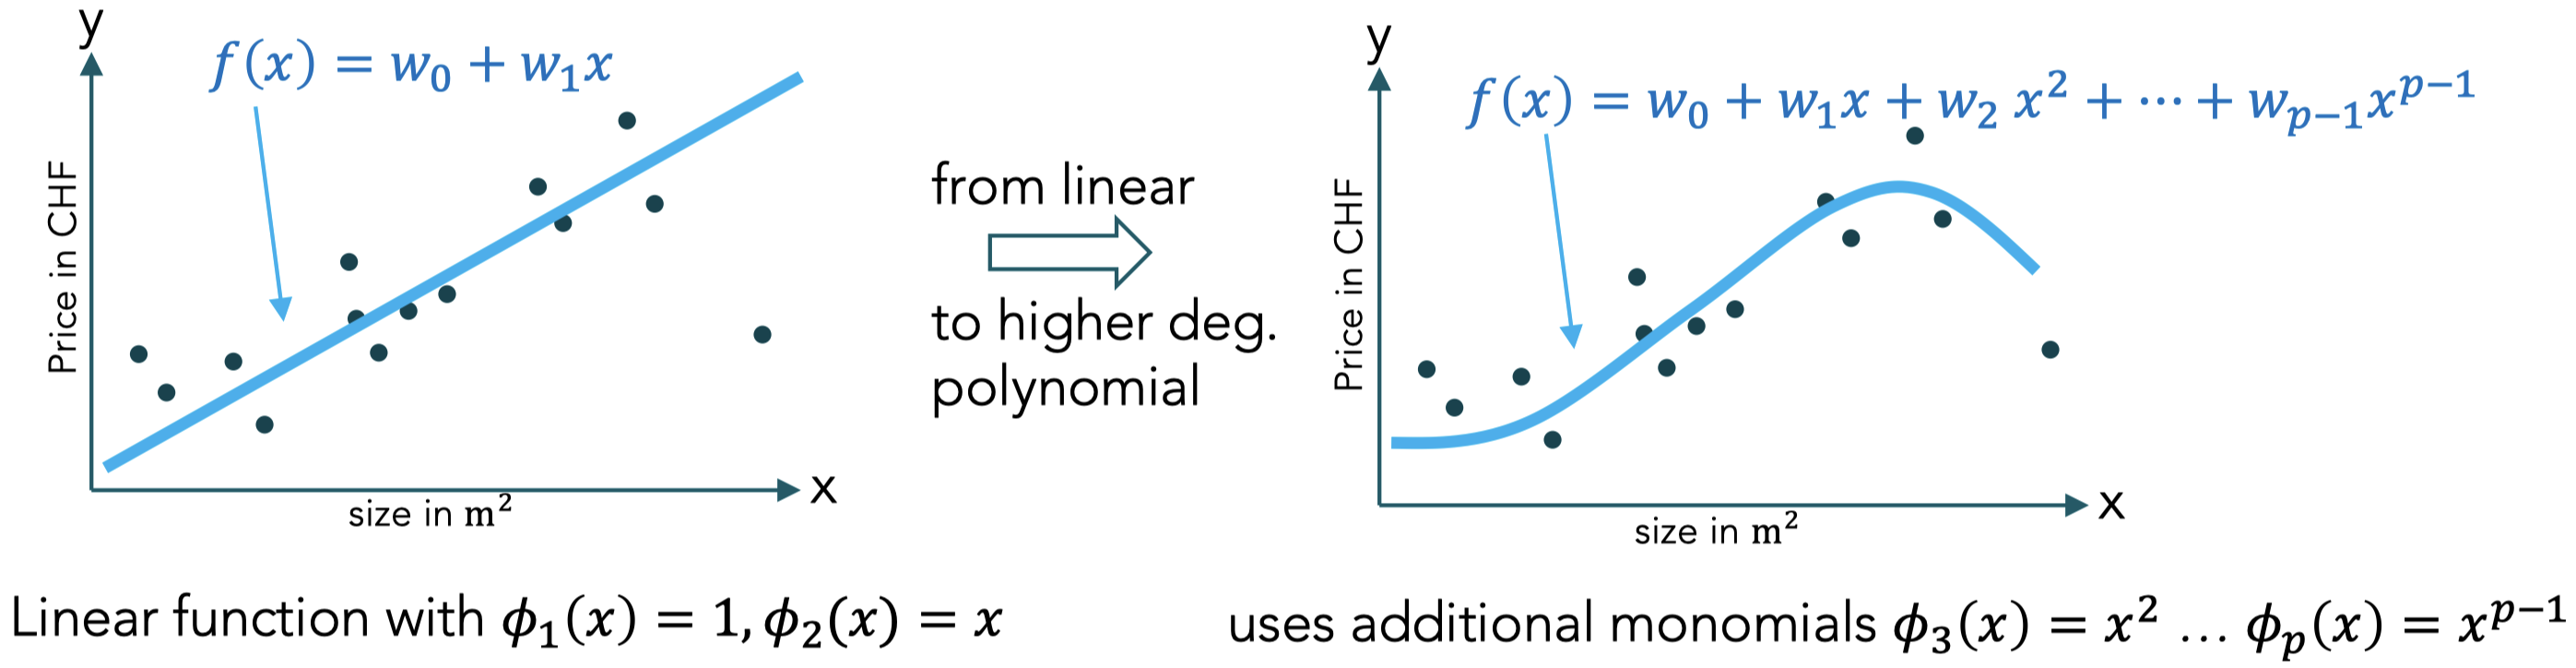
\includegraphics[width=15cm]{../images/IntroML_Fig2-3}
    \centering
\end{figure}

For the loss function we again consider the squared loss. We seek the minimizer of the square loss

\[
    \hat{f} = \text{argmin}_{f \in F_{\phi}} \frac{1}{n} \sum_{i = 1}^n (y_i - f(x_i))^2,
\]

this time in some fixed feature function space \(F_{\phi}\). This is equivalent to minimizing over vector \(w\):

\[
    \hat{w} = \text{argmin}_{w \in \mathbb{R}^p} L(w) = \frac{1}{n} \sum_{i = 1}^n (y_i - \sum_{j = 1}^p w_j \phi_j(x))^2
\]

We can rewrite the training loss \(L\) in matrix vector notation as follows:

\begin{figure}[H]
    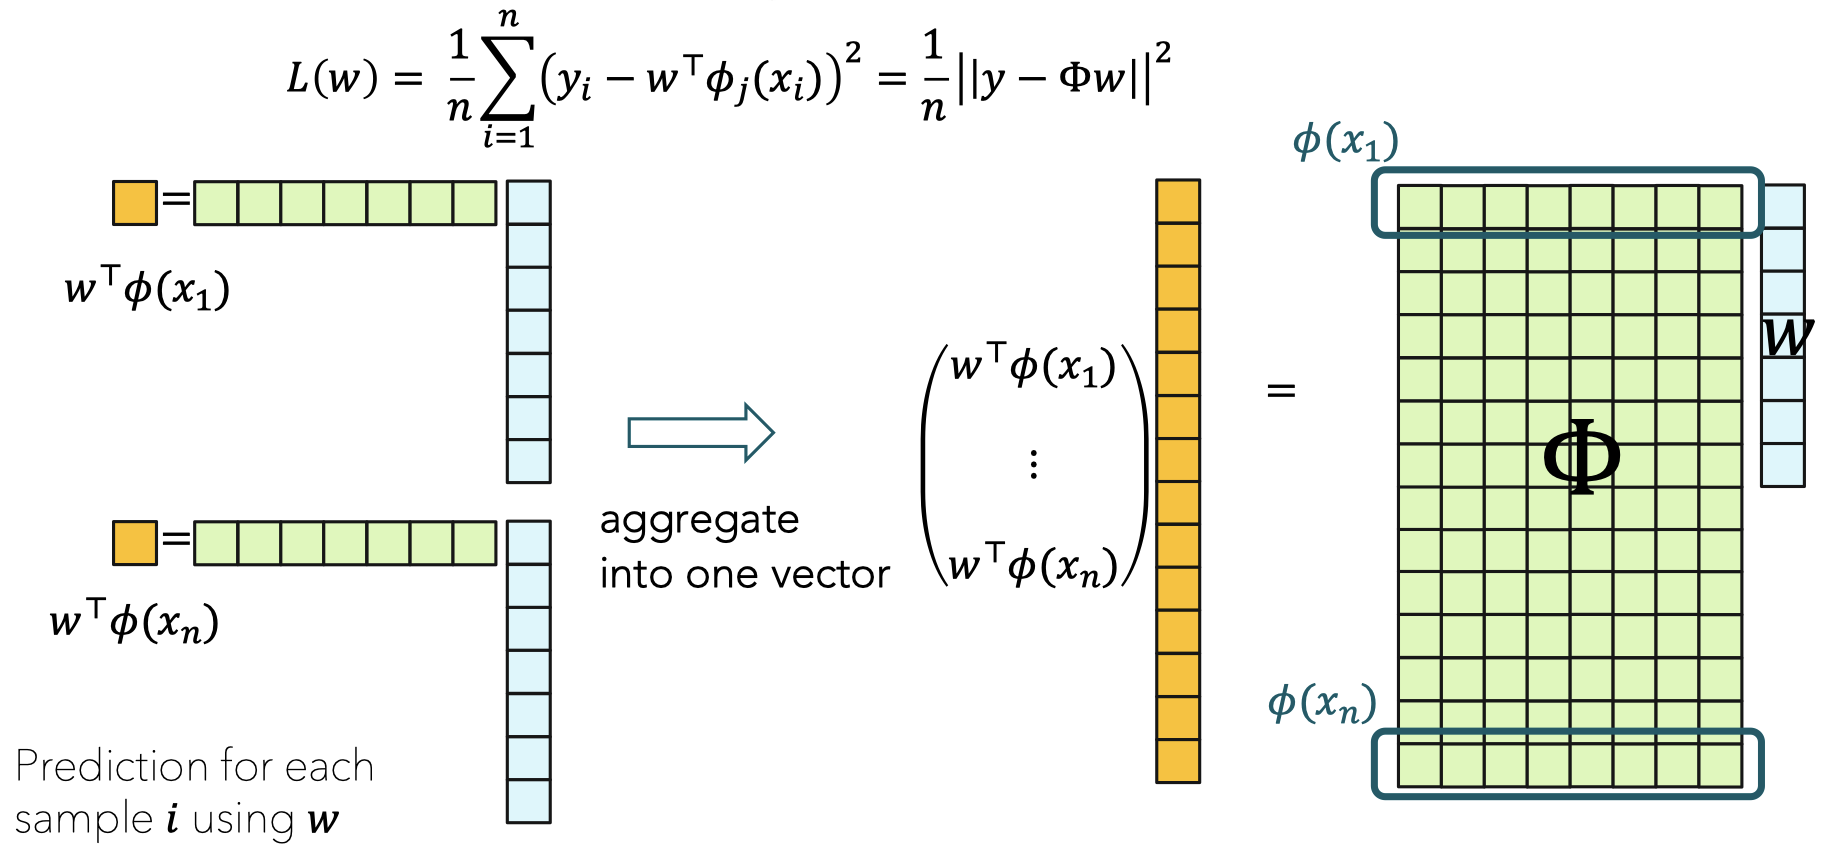
\includegraphics[width=13cm]{../images/IntroML_Fig2-4}
    \centering
\end{figure}

\end{document}